% https://www.researchgate.net/publication/331283709_A_portable_three-dimensional_LIDAR-based_system_for_long-term_and_wide-area_people_behavior_measurement
The build in a \acs{ros} package \mbox{hdl\_graph\_slam} is an open\hyp{}source \acs{3d} \acs{lidar} based \acs{slam}. The package has been tested in indoor and outdoor environments with a Velodyne HDL\hyp{}32E, a Velodyne VLP\hyp{}16, and a RobotSense RS\hyp{}\acs{lidar}\hyp{}16. The package is developed in 2019 by Kenji Koide, Jun Miura, and Emanuele Menegatti. It supports multiple constraints that can be individually be enabled or disabled, being odometry, loop closure, \acs{gps}, \acs{imu} acceleration, \acs{imu} orientation, and floor plane detection. \cite{koide2019portable}

This package was the first fully implemented \acs{slam} algorithm of this project. Not being able to deal with loop closes was its mayor flaw for this project. It worked perfectly when not disturbed, therefore it was not reliable.

\begin{figure}[!h]
  \centering
  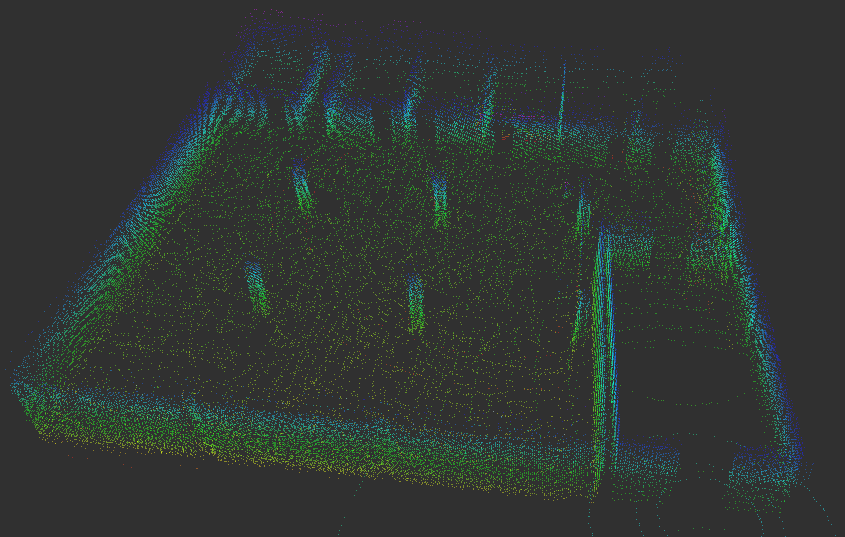
\includegraphics[width=\linewidth]{images/hdl_graph_slam_implementation.png}
  \caption{Implementation of hdl\_graph\_slam}
  \label{fig:hdl_graph_slam_implementation}
\end{figure}